\subsection{Overview}
In this paper, we introduce the range of oBERTa language models, an easy-to-use set of language models which allows Natural Language Processing (NLP) practitioners to obtain between 3.8 and 24.3 times faster models without expertise in model compression. Specifically, oBERTa extends existing work on pruning, knowledge distillation, and quantization and leverages frozen embeddings, improves distillation, and model initialization to deliver higher accuracy on a broad range of transfer tasks. In generating oBERTa, we explore how the highly optimized RoBERTa differs from the BERT for pruning during  pre-training and fine-tuning. We find it less amenable to compression during  fine-tuning. We explore the use of oBERTa on seven representative NLP tasks and find that the improved compression techniques allow a pruned oBERTa model to match the performance of BERT\textsubscript{base} and exceed the performance of Prune OFA Large on the SQUAD V1.1 Question Answering dataset, despite being 8x and 2x respectively faster in inference. We release our code, training regimes, and associated model for broad usage to encourage usage and experimentation. 
\subsection{Introduction}
\begin{figure}[!htb]
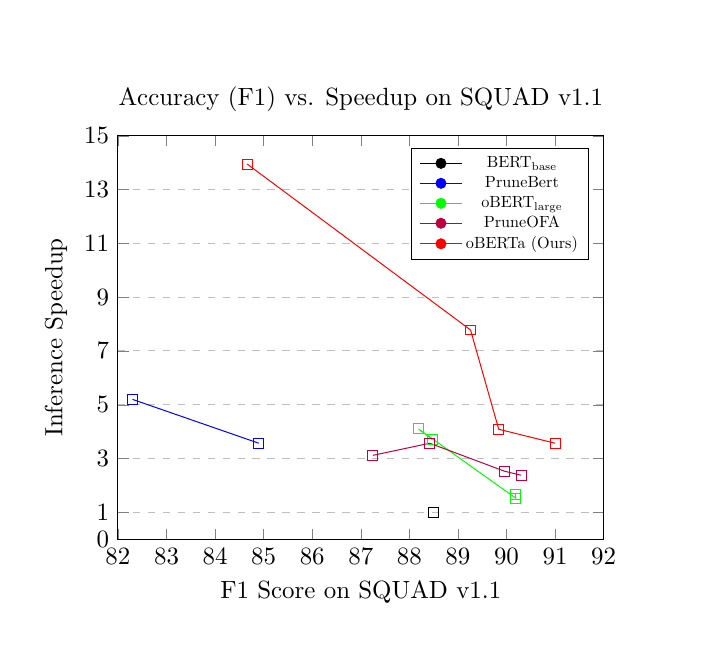
\begin{tikzpicture}
\scalebox{0.9}{
\begin{axis}[
    title={Accuracy (F1) vs. Speedup on SQUAD v1.1},
    xlabel={ F1 Score on SQUAD v1.1},
    ylabel={Inference Speedup},
    xmin=82, xmax=92,
    ymin=0 , ymax=15,
    xtick={82,83,84,85,86,87,88, 89, 90, 91,92},
    ytick={0,1,3,5,7,9,11,13,15},
    legend pos=north east,
    ymajorgrids=true,
    grid style=dashed,
    legend style={nodes={scale=0.65, transform shape}}, 
    legend image post style={mark=*}
]
\addplot[
    color=black,
    mark=square,
    ]
    coordinates {
    (88.5,1)
    };
\addplot[
    color=blue,
    mark=square,
    ]
    coordinates {
    (84.9,3.57)(82.3,5.2)
    };
\addplot[
    color=green,
    mark=square,
    ]
    coordinates {
    (88.47,3.71)(88.19,4.1)(90.19,1.53)(90.18, 1.68)
    };
\addplot[
    color=purple,
    mark=square,
    ]
    coordinates {
    (87.25,3.12)(88.42,3.57)(89.96, 2.53)(90.30, 2.38)
    };
\addplot[
    color=red,
    mark=square,
    ]
    coordinates {
    (91.0,3.57)(89.84,4.09)(89.26,7.78)(84.66,13.95)
    };
\legend{BERT\textsubscript{base} ,PruneBert,  oBERT\textsubscript{large} ,  PruneOFA, oBERTa (Ours)}
 \end{axis}}
\end{tikzpicture}
    \centering
    \caption{Performance of Sparse Language Models on the SQUAD V1.1 \cite{Rajpurkar2016SQuAD10} compared to an uncompressed BERT\textsubscript{base} \cite{Devlin2019BERTPO} with relation to realized inference improvements with regards to mean latency with a batch size of 1.}
    \label{fig:squadv1}
\end{figure}
The massive improvement in contextual word representations driven by the usage of the Transformer architecture \cite{Vaswani2017AttentionIA} has led to the wide-scale deployment of language models. These models are customized for various use cases and tasks like question answering, sentiment analysis, information retrieval, and document classification and deployed into general domains and specialized domains such as financial, medical, and legal. While these models are effective, they commonly contain hundreds of millions of parameters, which can lead to slow inference times without using specialized hardware accelerations like graphics processing units (GPU) or Tensor Processing Units (TPU). Without hardware acceleration, the inference on CPUs can be slow and impractical for real-world deployments.\\
Approaches such as knowledge distillation (KD) \cite{Hinton2015DistillingTK}, quantization \cite{Zafrir2019Q8BERTQ8}, and pruning \cite{Kurtic2022TheOB} have been leveraged to improve model efficiency and, when paired with specialized inference engines\footnote{https://github.com/neuralmagic/deepsparse}, it is possible to accelerate inference times on CPUs and GPUs significantly. While there has been substantial effort to create effective methods for compression \cite{Jiao2020TinyBERTDB, Sun2020MobileBERTAC} and improved model performance \cite{Liu2019RoBERTaAR}, general users of language models have been slower to adopt these methods. Years after its release, the original  BERT\textsubscript{base} uncased \cite{Devlin2019BERTPO} is still the most popular language model \footnote{Based on monthly downloads on the huggingface model hub in march 2023}, followed by the slightly compressed DistilBERT \cite{Sanh2019DistilBERTAD} for latency-sensitive deployments.
To enable broad adoption, regular users must be able to leverage more efficient language models without additional compression steps or tuning.\\
We present a case study on how to compress a language model for efficient CPU inference leveraging KD, structured pruning, unstructured sparsity, and quantization such that the compressed models can be applied to a broad range of natural language processing (NLP) tasks without expertise in compression of language models. \\
As part of this study, we release a set of efficient language models optimized to deliver the greatest improvement in inference while minimizing losses in accuracy. We then show how these models can be used for \textit{sparse transfer learning} \cite{Iofinova2021HowWD, Zafrir2021PruneOF} such that most compression happens during the pre-training stage. The pre-trained sparse models can be transferred to various NLP tasks, preserving sparsity without extensive optimization. Using these sparse transfer models and the DeepSparse inference engine, we show these sparse models can be fine-tuned to produce task-specific sparse models with minimal accuracy loss and result in greatly improved inference speeds with minimal accuracy loss.\\
As shown in figure \ref{fig:squadv1}, oBERTa provides state-of-the-art performance for sparse language models on the SQUAD v1.1 Question Answering dataset. oBERTa variants exceed the performance of BERT\textsubscript{base} despite being eight times faster, exceed the performance of Prune OFA\textsubscript{large} and oBERT\textsubscript{large} while being two to five times faster.
In this paper, we focus on the following research questions: 
\begin{itemize}
    \item RQ1: Is RoBERTa more sensitive to unstructured pruning than BERT?
    \item RQ2: What impact of using a larger teacher for KD during the pruning of language models? 
    \item RQ3: Can frozen embeddings improve the accuracy of pruned language models?
\end{itemize}As part of our experimentation, we release the associated models and the training regimes to aid reproducibility and encourage efficient inference models. \\
In summary, our contributions are as follows:
\begin{itemize}
    \item We provide a thorough case study on how to compress a less studied language model, RoBERTa \cite{Liu2019RoBERTaAR}, and evaluate performance on a set of seven NLP tasks finding that it is possible to effectively compress a language model without using its original pre-training dataset.
    \item We demonstrate the impact of varying the size of teachers in KD, freezing embeddings, and variations in learning rates when applied to sparse language models.
    \item We demonstrate that our compressed models can be leveraged to deliver accuracy of over 91\% on the popular SQUAD v1.1 \cite{Rajpurkar2016SQuAD10} Question Answering Task with nearly three times faster inference than the previous state-of-the-art uses of unstructured sparsity.
\end{itemize} 
\section{Background and Related work}
While many methods to improve model efficiency exist, the same goal generally underpins them: given an original model $\theta$ with an accuracy of $acc(\theta)$ and an inference cost of $c(\theta)$ minimize the inference cost. While the methods used for compression can be highly optimized and specialized, they can commonly be used together to deliver massive improvements in inference speeds with minimal losses in accuracy. \\
\textbf{Transformer Based Language Models} such as BERT \cite{Devlin2019BERTPO} and T5 \cite{Raffel2020ExploringTL} provide contextual language representations built on the Transformer architecture \cite{Vaswani2017AttentionIA} which can be specialized and adapted for specific tasks and domains \cite{Lee2020BioBERTAP}. Using these models, it becomes relatively easy to excel at a broad range of natural languages processing tasks such as Question Answering, Text Classification, and sentiment analysis. \\
\textbf{Unstructured Pruning} is a compression approach that removes individual weights or groups of weights in a model by applying a mask or setting the weight values to 0. This compression approach has been broadly studied in computer vision \cite{Han2015ADN}, and many methods can remove 70\% or more of model weights with little to no loss in accuracy. Models pruned can be 20x smaller in terms of pure model size and, when paired with a sparsity-aware inference engine such as DeepSparse \cite{deepsparse}, provide 3-5x speedups in inference throughput. Focused on language models, recent work has shown that it is possible to prune models during pre-training with little to no loss in accuracy \cite{Sanh2020MovementPA} \cite{Kurti2022TheOB} or during pre-training \cite{Zafrir2021PruneOF} and transfer to novel domains \cite{Campos2022SparseBERTSM} and datasets. \\
\textbf{Structured Pruning} is a compression approach that removes fundamental structural components in a language model such as individual attention heads \cite{Voita2019AnalyzingMS} or entire model layers such as transformer encoders \cite{sanh2019distilbert}. Structural pruning has become one of the most popular methods for inference optimization as it is easy to estimate the speedups and implement.\\
\textbf{Freezing Embeddings} as introduced by Devlin et al. \cite{Devlin2019BERTPO}, involves training the embedding layer of a language model and then toggling the ability to continue to optimize, or not, the values of in the embeddings as training continues. \\
\textbf{Knowledge Distillation} \cite{Hinton2015DistillingTK} is a training method where a model is not explicitly a compression method but a training method where a model, called the \textit{student} learns to emulate a \textit{teacher} model which is commonly larger or better performing. The loss extracted from the original training data in KD is augmented or replaced by KL divergence between the student and teacher model. \\
KD leverages the hardness parameter $h$ to control the mixture of regular and distillation loss (with a higher distillation favoring the KL divergence loss) and a temperature parameter $t$ to control the softness of the distribution. \\
As applied to language models, the approach has been used to improve the performance of structurally pruned language models resulting in models like DistilBERT \cite{sanh2019distilbert} and TinyBERT \cite{Jiao2020TinyBERTDB}. \\
\textbf{Quantization}Quantization precision for the model weights and activations to lower the computational requirements of model execution. While researchers have explored reducing representation to binary representations \cite{Pouransari2020LeastSB}, current hardware limits inference speedups to 8 or 4-bit representations. Quantization can be applied after the model is trained in a one-shot fashion, but this can lead to large losses in accuracy because of rounding errors. To avoid this pitfall, quantization Quantizations quantization-aware training (QAT), where the forward pass of the model is simulated with lower precision. In contrast, the backward pass happens in full precision. By using QAT models, learn to be robust to rounding errors and can result in Quantization having little to no loss in accuracy. In language models, research has produced quantized language models such as Q8BERT \cite{Zafrir2019Q8BERTQ8} and is commonly used in conjunction with structured and unstructured pruning \cite{Zafrir2021PruneOF} as a way of introducing compounding compression.\\
Other approaches such as early exiting \cite{Xin2020DeeBERTDE} or token pruning \cite{Kim2021LearnedTP} have also improved inference efficiency. Still, the inference improvements can be very dataset dependent and, as a result, out of our experimentation frame. \\
\section{Improving Sparse Transfer Learning}
While quantization and pruning have been well studied as applied to language models, work has studied the compression BERT\textsubscript{base} or BERT\textsubscript{large}. Despite existing research, we find that a clear case study that explores how best to create a family of compressed models is lacking, and this work seeks to remedy that. As part of our research, we compare the impact of varying pruning methods, pruning stage, teachers for KD, and freezing portions of the model as applied to the RoBERTa language model.\\
While performing task-specific compression allows NLP practitioners to broadly adopt improvements in inference efficiency, having access to pre-optimized models is key. We produce a family of 8 general purpose language models, collectively called oBERTa, which progressively get smaller and faster with minimal losses in accuracy. \\
The oBERTa models leverage a combination of structured and unstructured pruning to provide a set of compressed models which can meet a wide set of latency needs. This compression approach has not been extensively documented nor discussed. Our approach to producing the oBERTA models builds on prior explorations of the combination of compression methods \cite{Kurti2022TheOB} and addresses compression approaches in a staged manner as shown in Figure~\ref{fig:framework}.\\
First, we create three structural variants starting with a RoBERTa\textsubscript{base} model. The base uses 12 transformer layers, the medium uses 6, and the small uses 3. Following prior work, we select interleaved layers for the 6-layer model and the first, middle, and last layers for the 3-layer model. Then, each of these 3 models is further pre-trained using masked language modeling on the Wikipedia-Bookcorpus text dataset, leveraging KD from a  RoBERTa\textsubscript{large} teacher. After that, each model is pruned using gradual magnitude pruning (GMP) to a desired sparsity level (90\% and 95\%) during additional pre-training based on masked language modeling, similar to Zafir et al. \cite{Zafrir2021PruneOF}. Further background on the RoBERTA model and why we did not prune using the WebText corpus can be found in the appendix. \\
After pre-training, the sparsity profile is fixed, and models are fine-tuned and quantized on their target task with a small set of variable hyperparameters. Experimentation on the impact of larger teachers, frozen embeddings, and variations in pruning algorithms are discussed in subsequent portions of this work. 
\subsection{Downstream Compression}
We explore the impact of introducing unstructured sparsity during task-specific fine-tuning. We repeat each experiment with three different seeds and report the average F1 and Exact Match (EM) metrics in tables ~\ref{tab:OBS-downstream-squad} and \ref{tab:gmp-downstream-squad}. Following a basic hyperparameter sweep, our baseline RoBERTa\textsubscript{base} model achieves a performance of 83.95 EM and 91.13 F1 in the broadly used question-answering benchmark SQUAD V1.1 \cite{Rajpurkar2016SQuAD10}. \\
We also perform unstructured pruning varying the sparsity 50-95\% and the pruning method: GMP and OBS. We prune each model for eight epochs, followed by an additional two epochs to allow the network to stabilize and re-converge. Knowledge distillation is used during training with the dense baseline model as a teacher, hardness set to $1.0$ and temperature set to $5.0$.  Further hyperparameters are in the appendix \ref{sec:downstream}.\\
Table \ref{tab:Sparse-Benchmark} shows the impact of sparsity on BERT\textsubscript{base}, as reported by previous work. Comparing these results with tables \ref{tab:OBS-downstream-squad} and \ref{tab:gmp-downstream-squad}, we conclude that RoBERTa is more sensitive to pruning than BERT, although RoBERTa\textsubscript{base} pruned with OBS remains significantly more accurate than BERT\textsubscript{base} for the same level of sparsity.\\
Table~\ref{tab:OBS-downstream-squad} shows that pruning RoBERTA\textsubscript{base} to 90\% with OBS results in a relative drop in F1 of 1.59\%, which is three times the relative drop reported for BERT\textsubscript{base} with the same pruning algorithm.
Moreover, table~\ref{tab:gmp-downstream-squad} shows that RoBERTA\textsubscript{base} becomes very sensitive to pruning with GMP for sparsities above 85\%, with the relative drop in F1 increasing almost threefold between 85\% and 90\% sparsity.
We conjecture that RoBERTa is more sensitive to pruning than BERT because the latter is relatively under-trained \cite{Liu2019RoBERTaAR}, making the more optimized RoBERTa more sensitive to the loss in expressivity caused by pruning.
\begin{table}[!ht]
    \centering
    \tiny
    \begin{tabular}{|l|l|l|l|}
    \hline
        Model & Sparsity& F1& Impact  \\ \hline
         BERT\textsubscript{base} \cite{Devlin2019BERTPO} & 0 & 88.50 & N/A \\ \hline
         BERT\textsubscript{large} \cite{Devlin2019BERTPO} & 0 &  90.9 & N/A \\ \hline
         RoBERTa\textsubscript{base} \cite{Liu2019RoBERTaAR} & 0 & 91.13 & N/A \\ \hline
         RoBERTA\textsubscript{large} \cite{Liu2019RoBERTaAR} & 0 & 94.60 & N/A \\ \hline
         PruneBert\textsubscript{base} \cite{Sanh2020MovementPA} & 90 & 84.90 & -4.07 \%\\ \hline
         PruneOFA\textsubscript{large} \cite{Zafrir2021PruneOF}& 90 & 87.25 & -1.41 \% \\ \hline
         oBERT\textsubscript{large} \cite{Kurti2022TheOB} & 90 & 87.98 &  -0.58\%  \\ \hline
         $GMP_\star$\textsubscript{large} \cite{Kurtic2022GMPWG} & 90 & 86.7 & -2.03\% \\ \hline
    \end{tabular}
    \caption{Performance of existing dense and sparse language models on the SQUAD v1.1 Question Answering Dataset}
    \label{tab:Sparse-Benchmark}
\end{table}
\begin{table}[!ht]
    \centering
    \small
    \begin{tabular}{|l|l|l|l|l|}
    \hline
        Sparsity (\%) & EM & Impact & F1 & Impact \\ \hline
        50 & 84.80 & 1.01\% & 91.49 & 0.40\% \\ \hline
        60 & 84.64 & 0.82\% & 91.33 & 0.22\% \\ \hline
        70 & 84.42 & 0.56\% & 91.13 & 0.00\% \\ \hline
        80 & 84.64 & 0.82\% & 91.33 & 0.22\% \\ \hline
        85 & 82.89 & -1.26\% & 90.12 & -1.11\% \\ \hline
        90 & 82.48 & -1.75\% & 89.68 & -1.59\% \\ \hline
        95 & 79.01 & -5.89\% & 87.05 & -4.47\% \\ \hline
    \end{tabular}
    \caption{Impact of Sparsity introduced by OBS on the F1 and EM scores of pruned RoBERTa models on the SQUAD V1.1 Dataset}
    \label{tab:OBS-downstream-squad}
\end{table}

\begin{table}[!ht]
    \centering
    \small
    \begin{tabular}{|l|l|l|l|l|}
    \hline
        Sparsity (\%) & EM & Impact & F1 & Impact \\ \hline
        50 & 84.90 & 1.13\% & 91.46 & 0.36\% \\ \hline
        60 & 84.27 & 0.38\% & 90.91 & -0.24\% \\ \hline
        70 & 83.37 & -0.69\% & 90.30 & -0.91\% \\ \hline
        80 & 81.64 & -2.76\% & 88.86 & -2.49\% \\ \hline
        85 & 81.64 & -2.76\% & 88.86 & -2.49\% \\ \hline
        90 & 76.51 & -8.86\% & 84.90 & -6.83\% \\ \hline
        95 & 69.39 & -17.34\% & 79.35 & -12.93\% \\ \hline
    \end{tabular}
    \caption{Impact of Sparsity introduced by GMP on the F1 and EM scores of pruned RoBERTa models on the SQUAD V1.1 Dataset}
    \label{tab:gmp-downstream-squad}
\end{table}
\subsection{Upstream Compression}
Based on our fine-tuning experiments, achieving a high degree of sparsity on the RoBERTA model leads to improvements in performance, but there are greater than expected losses in accuracy. Additionally, such compression is task-specific and non-amortizable, so we explore how best to generate general pruned RoBERTa models. While we eventually apply the winning set of training combinations to all of our variants of oBERTa, we first seek to answer the following questions: Does GMP or OBS perform better during pretraining pruning? Does Freezing the Embeddings during pretraining pruning further improve performance? Does the use of larger teachers further improve performance? \\
We prune various models while varying individual variables during pretraining to evaluate these questions. We experiment by pruning an oBERTa\textsubscript{base} (12 layers) model to 90\% and 95\% sparsity on all non-embedding layers. All pretraining pruning happens using the Wikipedia-BookCorpus dataset, where we train for five epochs using a learning rate of 5e-5 and a batch size of 256 using 4 A100 GPUS. To evaluate the impact of these models, we evaluate performance on the previously used SQUAD v1.1 question-answering dataset, where we train with a fixed training regime of 10 epochs with a learning rate of 1.5e-4 based on the work of Kurtic et al. We train without KD for each finetuning run with an unpruned RoBERTa\textsubscript{base} or an unpruned RoBERTa\textsubscript{large}. Details for the hyperparameters used to train all teacher models can be found in the appendix \ref{sec:TeacherStats}.  \\
\begin{table}[!ht]
    \centering
    \tiny
    \scalebox{0.65}{
    \begin{tabular}{|l|*4l|*4l|}
    \toprule
         &  \multicolumn{4}{l}{GMP} & \multicolumn{4}{l}{OBS} \\ 
        \toprule
        Model & F1 & Impact & EM & Impact & F1 & Impact & EM & Impact \\ \hline
        RoBERTA\textsubscript{base} & 92.18 & 0.00\% & 85.59 & 0.00\% & 92.18 & 0.00\% & 85.59 & 0.00\% \\ \hline
        oBERTa 90\% No KD & 88.34 & -4.17\% & 80.19 & -6.31\% & 87.72 & -4.83\% & 79.35 & -7.29\% \\ \hline
        oBERTa 90\% RoBERTA\textsubscript{base} KD & 88.75 & -3.72\% & 81.35 & -4.95\% & 88.60 & -3.88\% & 81.37 & -4.93\% \\ \hline
        oBERTa 90\% RoBERTA\textsubscript{large} KD & 89.65 & -2.75\% & 83.12 & -2.88\% & 89.63 & -2.76\% & 82.94 & -3.09\% \\ \hline
        oBERTa 95\% No KD & 86.58 & -6.07\% & 78.81 & -7.92\% & 84.90 & -7.90\% & 76.82 & -10.25\% \\ \hline
        oBERTa 95\% RoBERTA\textsubscript{base} KD & 86.99 & -5.63\% & 79.41 & -7.22\% & 86.14 & -6.55\% & 78.63 & -8.13\% \\ \hline
        oBERTa 95\% RoBERTA\textsubscript{large} KD & 87.60 & -4.97\% & 80.44 & -6.01\% & 86.14 & -6.55\% & 79.84 & -6.72\% \\ \hline
        \bottomrule
    \end{tabular}}
    \caption{Impact on F1 of SQUAD V1.1 of using OBS vs. GMP as the pruning method during pretraining. Impact measures the relative loss in performance vs. the unpruned RoBERTa\textsubscript{base} baseline.}
    \label{tab:OBS-vs-GMP-hard1.0}
\end{table}
Comparing the use of OBS vs. GMP as shown in table \ref{tab:OBS-vs-GMP-hard1.0}, we can see that GMP consistently outperforms OBS. This is the opposite of what is seen when pruning downstream or, in prior work, pruning BERT. We attribute this inversion to not using the web-text dataset and leveraging the Wikipedia-book-corpus instead. We believe that without access to the original training corpus OBS is leading to overfitting of the sparse models, a dataset that is not its intended target. \\
\begin{table}[!ht]
    \centering
    \small
    \scalebox{0.57}{
    \begin{tabular}{|l|*4l|*4l|}
    \toprule
         &  \multicolumn{4}{l}{Hardness 0.5} & \multicolumn{4}{l}{Hardness 1.0} \\ 
        \toprule
        Model & F1 & Impact & EM & Impact & F1 & Impact & EM & Impact \\ \hline
         RoBERTA\textsubscript{base} & 92.18 & 0.00\% & 85.59 & 0.00\% & 92.18 & 0.00\% & 85.59 & 0.00\% \\ \hline
        oBERTa 90\% No KD & 88.21 & -4.31\% & 80.19 & -6.31\% & 88.34 & -4.17\% & 80.19 & -6.31\% \\ \hline
        oBERTa 90\% Base KD & 89.19 & -3.25\% & 81.74 & -4.50\% & 88.75 & -3.72\% & 81.35 & -4.95\% \\ \hline
        oBERTa 90\% Large KD & 90.14 & -2.21\% & 83.51 & -2.43\% & 89.65 & -2.75\% & 83.12 & -2.88\% \\ \hline
        oBERTa-95 No KD & 85.82 & -6.90\% & 77.77 & -9.14\% & 86.58 & -6.07\% & 78.81 & -7.92\% \\ \hline
        oBERTa-95 Base KD & 86.98 & -5.64\% & 79.23 & -7.43\% & 86.99 & -5.63\% & 79.41 & -7.22\% \\ \hline
        oBERTa-95 Large KD & 87.66 & -4.91\% & 80.40 & -6.07\% & 87.60 & -4.97\% & 80.44 & -6.01\% \\ \hline
        \bottomrule
    \end{tabular}}
    \caption{Impact on F1 of SQUAD V1.1 by hardness in KD during pretraining pruning. Impact measures the relative loss in performance vs. the unpruned RoBERTa\textsubscript{base} baseline.}
    \label{tab:hardness-oberta}
\end{table}
  Evaluating the impact of variations in the hardness  of KD as shown in table \ref{tab:hardness-oberta}, there is a bit more of a muted set of conclusions. The 95\% sparse models perform better with a hardness of 1.0, while the 90\% models do better with a hardness of 0.5. Given that our goal is to preserve most of the RoBERTa model without actually using its large dataset, we set our hardness to 1.0 as it keeps the model from explicitly learning the new dataset. \\
\begin{table}[!ht]
    \centering
    \small
    \scalebox{0.5}{
    \begin{tabular}{|l|*4l|*4l|}
    \toprule
          &  \multicolumn{4}{l}{Frozen Embeddings} & \multicolumn{4}{l}{Trained Embeddings} \\ 
        \midrule
        Model & F1 & Impact & EM & Impact & F1 & Impact & EM & Impact \\ \hline
        RoBERTa\textsubscript{base} & 92.18 & 0.00\% & 85.59 & 0.00\% & 92.18 & 0.00\% & 85.59 & 0.00\% \\ \hline
        oBERTa\textsubscript{base} 90\% no KD & 87.71 & -4.85\% & 79.62 & -6.98\% & 88.21 & -4.31\% & 80.19 & -6.31\% \\ \hline
        oBERTa\textsubscript{base} 90\% RoBERTa\textsubscript{base} KD & 89.7 & -2.69\% & 81.74 & -4.50\% & 89.19 & -3.24\% & 83.07 & -2.94\% \\ \hline
        oBERTa\textsubscript{base} 90\% RoBERTa\textsubscript{large} KD & 89.59 & -2.81\% & 82.98 & -3.05\% & 90.14 & -2.21\% & 83.51 & -2.43\% \\ \hline
        \bottomrule
    \end{tabular}}
    \caption{Impact on F1 of SQUAD V1.1 with respect to the use of frozen embeddings or not during pretraining pruning. Impact measures the relative loss in performance vs. the unpruned RoBERTa\textsubscript{base} baseline.}
    \label{tab:freeze-embd-oberta}
\end{table}
When we evaluate the impact of freezing embeddings during pre-training, as shown in table \ref{tab:freeze-embd-oberta}, we find strong evidence that using frozen embeddings consistently leads to worse performance and, as a result, does not freeze embeddings during our model pruning. Looking at the impact of varying the size of the teacher for pretraining KD as shown in table \ref{tab:upsteam-teach}, we unsurprisingly find clear evidence that using a larger teacher during pretraining pruning leads to improvements in performance. \\
\begin{table}[!ht]
    \centering
    \small
    \scalebox{0.55}{
    \begin{tabular}{|l|*4l|*4l|}
    \toprule
          &  \multicolumn{4}{l}{Base Upstream Teacher} & \multicolumn{4}{l}{Large Upstream Teacher} \\ 
        \midrule
        Model & F1 & Impact & EM & Impact & F1 & Impact & EM & Impact \\ \hline
        RoBERTA\textsubscript{base} & 92.18 & 0.00\% & 85.59 & 0.00\% & 92.18 & 0.00\% & 85.59 & 0.00\% \\ \hline
        oBERTa 90\% no KD  & 88.34 & -4.17\% & 80.59 & -5.84\% & 88.1 & -4.43\% & 80.06 & -6.46\% \\ \hline
        oBERTa 90\% Base KD & 88.75 & -3.72\% & 81.35 & -4.95\% & 89.22 & -3.21\% & 82.02 & -4.17\% \\ \hline
        oBERTa 90\% Large KD & 89.65 & -2.74\% & 83.12 & -2.89\% & 89.98 & -2.39\% & 83.14 & -2.86\% \\ \hline
        \bottomrule
    \end{tabular}}
    
    \caption{Impact on F1 of SQUAD V1.1 with respect variation is the size of the teacher in KD during pretraining pruning. Impact measures the relative loss in performance vs. the unpruned RoBERTa\textsubscript{base} baseline.}
    \label{tab:upsteam-teach}
\end{table}
Using these experiments, we generate the recipe, which we then use to create the many variants of oBERTa. We pre-train models using KD using a RoBERTa\textsubscript{large} teacher with a hardness of 1.0; we do not freeze the embeddings and use GMP to prune.
\section{Experimental Results}
Based on the aforementioned experiments, we generate 8 variants of oBERTa, each with a different size and sparsity profile; details can be found in table \ref{tab:oberta-model-info}. Within this table, we report the impact on the model size as measured by the raw and compressed size of the ONNX \footnote{https://onnx.ai/} model file. Embeddings are unpruned and each layer is pruned to the target sparsity profile independent of the rest of the model. As a result, the overall sparsity profile may vary as modules in the network may not be able to reach exactly 90\% or 95\% sparsity. \\
Using these \textit {inference-optimized} models, we evaluate their \textit{sparse transfer} performance by finetuning these models on their target task using a fixed training regime and minor hyperparameter exploration. For each task, we train them for 10 epochs or 20 (10 of which are Quantization Aware Training), with the longer schedule being reserved for models which are being quantized.  \\
We evaluate performance on a benchmark of diverse NLP tasks ranging from question answering, sentiment analysis, document classification, token classification, and text classification. For question answering, we leverage the SQuAD v1.1 \cite{Rajpurkar2016SQuAD10} and SQuAD V2.0 \cite{Rajpurkar2018KnowWY} datasets. We leverage the SST-2 \cite{socher-etal-2013-recursive} dataset for sentiment analysis. For text classification, we use the Quora Duplicate Query Detection (QQP) \cite{sambitsekhar_2017} and the MNLI \cite{N18-1101} datasets. We leverage the IMDB \cite{maas-EtAl:2011:ACL-HLT2011} dataset for document classification and CONLL2003 \cite{tjong-kim-sang-de-meulder-2003-introduction} for token classification.\\ 
Looking at performance on question answering as shown in table \ref{tab:sparse-transfer-squad} and \ref{tab:sparse-transfer-squad2}.
\begin{table}[!ht]
    \centering
    \tiny
    \scalebox{0.8}{
    \begin{tabular}{|l|*3l|*3l|}
    \toprule
         &  \multicolumn{3}{l}{Sparse Transfer} & \multicolumn{3}{l}{Sparse Transfer With Quantization} \\ 
        \midrule
        model & F1 & Recovery & EM & F1 & Recovery & EM \\ \hline
        oBERTa\textsubscript{base} & 92.15 & 100.00\% & 85.78 & 93.18 & 101.11\% & 87.29 \\ \hline
        oBERTa\textsubscript{base} 90$\backslash$\% & 90.95 & 98.69\% & 84.42 & 89.46 & 97.08\% & 82.61 \\ \hline
        oBERTa\textsubscript{base} 95$\backslash$\% & 89.84 & 97.49\% & 83.08 & 89.23 & 96.83\% &  81.12\\ \hline
        oBERTa\textsubscript{MEDIUM} & 90.37 & 98.06\% & 83.84 & 83.77 & 90.91\% & 90.37 \\ \hline
        oBERTa\textsubscript{MEDIUM} 90$\backslash$\% & 89.26 & 96.86\% & 82.18 & 88.65 & 96.20\% & 81.88 \\ \hline
        oBERTa\textsubscript{SMALL} & 84.87 & 92.09\% & 76.55 & 84.82 & 92.05\% & 76.77 \\ \hline
        oBERTa\textsubscript{SMALL} 90$\backslash$\% & 84.66 & 91.87\% & 76.18 & 82.18 & 92.18\% & 74.21\\ 
        \bottomrule
    \end{tabular}}
   
    \caption{Sparse Transfer performance of the oBERTA family on the SQUAD V1.1 dataset. The sparse transfer was performed over 10 epochs and sparse transfer with quantization over 20. Recovery is based on the relative performance of the unpruned oBERTa\textsubscript{base}. }
    \label{tab:sparse-transfer-squad}
\end{table}
\begin{table}[!ht]
    \centering
    \begin{tiny}
    \scalebox{0.8}{
    \begin{tabular}{|l|*3l|*3l|}
    \toprule
         &  \multicolumn{3}{l}{Sparse Transfer} & \multicolumn{3}{l}{Sparse Transfer With Quantization} \\ 
        \midrule
         model & F1 & Recovery & EM & F1 & Recovery & EM \\ \hline
        oBERTa\textsubscript{base} & 82.77 & 100.00\% & 79.56 & 85.298 & 103.06\% & 82.347 \\ \hline
        oBERTa\textsubscript{base} 90$\backslash$\% & 81.33 & 98.26\% & 78.27 & 81.43 & 98.38\% & 78.92 \\ \hline
        oBERTa\textsubscript{base} 95$\backslash$\% & 77.98 & 94.22\% & 74.67 & 78.09 & 94.35\% & 74.82 \\ \hline
        oBERTa\textsubscript{MEDIUM} & 77.51 & 93.65\% & 74.25 & 78.137 & 94.41\% & 75.179 \\ \hline
        oBERTa\textsubscript{MEDIUM} 90$\backslash$\% & 76.64 & 92.60\% & 73.34 & 76.24 & 92.11\% & 73.51 \\ \hline
        oBERTa\textsubscript{SMALL} & 71.54 & 86.44\% & 67.93 & 71.591 & 86.50\% & 68.087 \\ \hline
        oBERTa\textsubscript{SMALL} 90$\backslash$\% & 70.79 & 85.53\% & 67.31 & 69.35 & 87.79\% & 65.21 \\ \hline
        \bottomrule
    \end{tabular}}
    \end{tiny}
    \caption{Sparse Transfer performance of the oBERTA family on the SQUAD V2.0 dataset. The sparse transfer was performed over 10 epochs, and sparse transfer with quantization over 20. Recovery is based on the relative performance of the unpruned oBERTa\textsubscript{base}. }
    \label{tab:sparse-transfer-squad2}
\end{table}
Moving to text classification on QQP and MNLI as shown in tables \ref{tab:sparse-transfer-qqp} and \ref{tab:sparse-transfer-MNLI}
\begin{table}[!ht]
    \centering
    \begin{tiny}
    \scalebox{0.70}{
    \begin{tabular}{|l|*3l|*3l|}
    \toprule
         &  \multicolumn{3}{l}{Sparse Transfer} & \multicolumn{3}{l}{Sparse Transfer With Quantization} \\ 
        \midrule
         model & Accuracy & Recovery &Accuracy(MM) & Accuracy & Recovery & Accuracy(MM) \\ \hline
        oBERTa\textsubscript{base} & 87.88\% & 100.00\% & 87.57\% & 88.06\% & 100.20\% & 88.01\% \\ \hline
        oBERTa\textsubscript{base} 90\% & 85.17\% & 96.91\% & 84.73\% & 85.09\% & 96.83\% & 84.76\% \\ \hline
        oBERTa\textsubscript{base} 95\% & 84.32\% & 95.95\% & 84.08\% & 83.73\% & 95.28\% & 83.83\% \\ \hline
        oBERTa\textsubscript{MEDIUM} & 85.29\% & 97.05\% & 85.17\% & 83.62\% & 95.15\% & 83.74\% \\ \hline
        oBERTa\textsubscript{MEDIUM} 90\% & 81.61\% & 92.87\% & 81.32\% & 82.37\% & 93.73\% & 81.79\% \\ \hline
        oBERTa\textsubscript{SMALL} & 80.80\% & 91.95\% & 81.55\% & 81.10\% & 92.29\% & 81.51\% \\ \hline
        oBERTa\textsubscript{SMALL} 90\% & 79.23\% & 90.15\% & 79.24\% & 79.14\% & 90.06\% & 79.42\% \\ \hline
        \bottomrule
    \end{tabular}}
    \end{tiny}
    \caption{Sparse Transfer performance of the oBERTA family on the MNLI dataset. Sparse transfer was performed over 10 epochs and sparse transfer with quantization over 20. Recovery is based on the relative performance of the unpruned oBERTa\textsubscript{base}. }
    \label{tab:sparse-transfer-MNLI}
\end{table}
\begin{table}[!ht]
    \centering
    \begin{tiny}
    \scalebox{0.6}{
    \begin{tabular}{|l|*4l|*4l|}
    \toprule
         &  \multicolumn{4}{l}{Sparse Transfer} & \multicolumn{4}{l}{Sparse Transfer With Quantization} \\ 
        \midrule
        model & Accuracy & Recovery & F1 & Combined & Accuracy & Recovery & F1 & Combined \\ \hline
        oBERTa\textsubscript{base} & 91.52\% & 100.00\% & 90.09\% & 88.66\% & 89.86\% & 98.18\% & 88.12\% & 86.73\% \\ \hline
        oBERTa\textsubscript{base} 90\% & 91.01\% & 99.44\% & 89.47\% & 87.92\% & 91.21\% & 99.66\% & 89.68\% & 88.16\% \\ \hline
        oBERTa\textsubscript{base} 95\% & 90.85\% & 99.26\% & 89.21\% & 87.58\% & 90.72\% & 99.12\% & 89.08\% & 0.87\% \\ \hline
        oBERTa\textsubscript{MEDIUM} & 91.35\% & 99.81\% & 89.90\% & 88.44\% & 91.33\% & 99.79\% & 89.80\% & 88.28\% \\ \hline
        oBERTa\textsubscript{MEDIUM} 90\% & 90.48\% & 98.86\% & 88.85\% & 87.21\% & 90.60\% & 99.00\% & 89.01\% & 87.42\% \\ \hline
        oBERTa\textsubscript{SMALL} & 90.72\% & 99.13\% & 89.21\% & 87.71\% & 89.74 & 98.06\% & 87.99 & 86.25 \\ \hline
        oBERTa\textsubscript{SMALL} 90\% & 89.74\% & 98.06\% & 87.99\% & 86.25\% & 89.73 & 98.04\% & 87.98 & 86.08\\
        \bottomrule
    \end{tabular}}
    \end{tiny}
    \caption{Sparse Transfer performance of the oBERTA family on the QQP dataset. The sparse transfer was performed over ten epochs, and sparse transfer with quantization over 20. Recovery is based on the relative performance of the unpruned oBERTa\textsubscript{base}.}
    \label{tab:sparse-transfer-qqp}
\end{table}
Shifting focus to document classification as shown in table \ref{tab:sparse-transfer-imdb} and sentiment analysis in \ref{tab:sparse-transfer-SST2}
\begin{table}[!ht]
    \centering
    \begin{tiny}
    \scalebox{0.95}{
    \begin{tabular}{|l|*2l|*2l|}
    \toprule
         &  \multicolumn{2}{l}{Sparse Transfer} & \multicolumn{2}{l}{Sparse Transfer With Quantization} \\ 
        \midrule
        model & Accuracy & Recovery & Accuracy & Recovery \\ \hline
        oBERTa\textsubscript{base} & 95.24\% & 100.00\% & 95.44\% & 100.21\% \\ \hline
        oBERTa\textsubscript{base} 90\% & 93.64\% & 98.32\% & 93.28 & 97.94\% \\ \hline
        oBERTa\textsubscript{base} 95\% & 93.48\% & 98.15\% & 92.80& 97.23\% \\ \hline
        oBERTa\textsubscript{MEDIUM} & 93.36\% & 98.03\% & 94.08 & 98.78\% \\ \hline
        oBERTa\textsubscript{MEDIUM} 90\% & 92.24\% & 96.85\% & 92.08& 96.69\% \\ \hline
        oBERTa\textsubscript{SMALL} & 93.04\% & 97.69\% & 92.52 & 97.15\% \\ \hline
        oBERTa\textsubscript{SMALL} 90\% & 91.60\% & 96.18\% & 91.28 & 95.84\% \\
        \bottomrule
    \end{tabular}}
    \end{tiny}
    \caption{Sparse Transfer performance of the oBERTA family on the IMDB dataset. The sparse transfer was performed over ten epochs, and sparse transfer with quantization over 20. Recovery is based on the relative performance of the unpruned oBERTa\textsubscript{base}. }
    \label{tab:sparse-transfer-imdb}
\end{table}
\begin{table}[!ht]
    \centering
    \begin{tiny}
    \scalebox{0.95}{
    \begin{tabular}{|l|*2l|*2l|}
    \toprule
         &  \multicolumn{2}{l}{Sparse Transfer} & \multicolumn{2}{l}{Sparse Transfer With Quantization} \\ 
        \midrule
        model & Accuracy & Recovery & Accuracy & Recovery \\ \hline
        oBERTa\textsubscript{base} & 94.60 & 100.00\% & 92.66 & 97.95\% \\ \hline
        oBERTa\textsubscript{base} 90\% & 92.78 & 98.08\% & 92.546 & 97.83\% \\ \hline
        oBERTa\textsubscript{base} 95\% & 91.51 & 96.74\% & 91.399 & 96.62\% \\ \hline
        oBERTa\textsubscript{MEDIUM} & 92.89 & 98.19\% & 91.06 & 96.26\% \\ \hline
        oBERTa\textsubscript{MEDIUM} 90\% & 88.76 & 93.83\% & 89.91 & 95.04\% \\ \hline
        oBERTa\textsubscript{SMALL} & 90.48 & 95.64\% & 91.28 & 96.49\% \\ \hline
        oBERTa\textsubscript{SMALL} 90\% & 89.34 & 94.44\% & 88.65 & 93.71\% \\ 
        \bottomrule
    \end{tabular}}
    \end{tiny}
    \caption{Sparse Transfer performance of the oBERTA family on the SST-2 dataset. The sparse transfer was performed over ten epochs, and sparse transfer with quantization over 20. Recovery is based on the relative performance of the unpruned oBERTa\textsubscript{base}. }
    \label{tab:sparse-transfer-SST2}
\end{table}
Finally, looking at performance on token classification as shown in table \ref{tab:sparse-transfer-conll2003} 
\begin{table}[!ht]
    \centering
    \begin{tiny}
    \scalebox{0.75}{
    \begin{tabular}{|l|*3l|*3l|}
    \toprule
         &  \multicolumn{3}{l}{Sparse Transfer} & \multicolumn{3}{l}{Sparse Transfer With Quantization} \\ 
        \midrule
        model & Accuracy & Recovery & F1 & Accuracy & Recovery & F1 \\ \hline
        oBERTa\textsubscript{base} & 99.26\% & 100.00\% & 95.51\% & 99.30\% & 100.05\% & 95.98\% \\ \hline
        oBERTa\textsubscript{base} 90\% & 99.11\% & 99.85\% & 94.98\% & 99.05\% & 99.79\% & 94.51\% \\ \hline
        oBERTa\textsubscript{base} 95\% & 98.89\% & 99.63\% & 93.32\% & 98.75\% & 99.48\% & 92.61\% \\ \hline
        oBERTa\textsubscript{MEDIUM} & 99.04\% & 99.77\% & 94.39\% & 99.18\% & 99.92\% & 95.15\% \\ \hline
        oBERTa\textsubscript{MEDIUM} 90\% & 98.79\% & 99.53\% & 93.31\% & 98.73\% & 99.46\% & 92.70\% \\ \hline
        oBERTa\textsubscript{SMALL} & 99.01\% & 99.75\% & 94.00\% & 98.98\% & 99.72\% & 94.13\% \\ \hline
        oBERTa\textsubscript{SMALL} 90\% & 98.47\% & 99.20\% & 91.13\% & 98.25\% & 98.98\% & 89.79\% \\ 
        \bottomrule
    \end{tabular}}
    \end{tiny}
    \caption{Sparse Transfer performance of the oBERTA family on the CONLL-2003 dataset. The sparse transfer was performed over ten epochs, and sparse transfer with quantization over 20. Recovery is based on the relative performance of the unpruned oBERTa\textsubscript{base}. }
    \label{tab:sparse-transfer-conll2003}
\end{table}

\subsection{Inference Benchmark}
To evaluate the performance of our inference-optimized models, we benchmark performance using the popular DeepSparse library version 1.3.2 \footnote{pip install deepsparse==1.3.2} and an Intel Xeon Gold 6238R Processor. Performance is measured using models that have been \textit{sparse-transferred} to the SQuAD v1.1 dataset and exported to a standard ONNX model format. Benchmarks are run on 4 and 24 cores and a sequence length of 384 with batch sizes of 1, 16, and 64. For each model, the benchmark is run for 60 seconds with a warm-up period of 10 seconds, and we report the throughput (items per second) and the mean, median, and standard deviation per item latency. 
\begin{table}[!ht]
    \centering
    \begin{tiny}
    \scalebox{0.85}{
    \begin{tabular}{|l|*3l|*3l|}
    \toprule
         &  \multicolumn{3}{l}{24 Cores} & \multicolumn{3}{l}{4 Cores} \\ 
        \midrule
        Model & BS 1 & BS 16 & BS 64 &  BS 1 & BS 16 & BS 64 \\
        \midrule
        oBERTa\textsubscript{base} & 1.00 & 1.00 & 1.00 & 1.00 & 1.00 & 1.00 \\ \hline
        oBERTa\textsubscript{base} Quantized & 3.10 & 4.29 & 4.46 & 4.09 & 4.31 & 4.32 \\ \hline
        oBERTa\textsubscript{base} 90\% & 3.29 & 3.80 & 3.80 & 3.60 & 3.34 & 3.40 \\ \hline
        oBERTa\textsubscript{base} 90\% Quantized & 4.12 & 7.05 & 7.37 & 7.67 & 7.59 & 7.40 \\ \hline
        oBERTa\textsubscript{base} 95\% & 8.72 & 4.56 & 4.65 & 4.12 & 3.85 & 4.37 \\ \hline
        oBERTa\textsubscript{base} 95\% Quantized & 4.73 & 8.22 & 8.56 & 9.41 & 9.06 & 8.68 \\ \hline
        oBERTa\textsubscript{MEDIUM} & 1.96 & 1.99 & 1.99 & 1.96 & 1.99 & 2.02 \\ \hline
        oBERTa\textsubscript{MEDIUM} Quantized & 6.20 & 8.04 & 8.44 & 8.43 & 8.33 & 8.45 \\ \hline
        oBERTa\textsubscript{MEDIUM} 90\%   & 6.35 & 7.41 & 6.84 & 7.83 & 6.56 & 6.72 \\ \hline
        oBERTa\textsubscript{MEDIUM} 90\% Quantized  & 8.94 & 12.86 & 13.65 & 14.99 & 14.81 & 14.95 \\ \hline
        oBERTa\textsubscript{SMALL} & 3.89 & 3.96 & 3.99 & 3.95 & 3.97 & 4.03 \\ \hline
        oBERTa\textsubscript{SMALL} Quantized & 12.47 & 14.12 & 14.08 & 15.50 & 15.48 & 15.70 \\ \hline
        oBERTa\textsubscript{SMALL} 90\% & 12.22 & 14.40 & 14.67 & 14.05 & 14.19 & 14.13 \\ \hline
        oBERTa\textsubscript{SMALL} 90\% Quantized & 16.21 & 21.35 & 23.96 & 29.77 & 27.14 & 27.58 \\ \hline
        \bottomrule
    \end{tabular}}
    \end{tiny}
    \caption{Latency reduction of the oBERTa family concerning the unpruned oBERTa\textsubscript{base} as measured on 24 and 4 cores. Speedup is measured relative to the latency reduction in MS/batch, and BS refers to batch size.}
    \label{tab:inference-bench}
\end{table}
We present a set of summary statistics of relative speedup across batch sizes and inference server configurations as shown in table \ref{tab:inference-bench}. Full inference performance results can be found in the appendix. In analyzing performance, we can see that the introduction of quantization to a dense model delivers roughly a 4x speedup while quantization on sparse models is closer to 2x. With the introduction of sparsity, 90\% leads to slightly under 4x speedup, while 95\% leads to slightly over 4x. The impact of structural pruning is roughly equivalent to the size of the as a 6-layer model is two times faster than a 12-layer, and a 3-layer model is four times faster. Since these different compression forms are additive, we can see that a small (3-layer) 90\% quantized model performance is ~24x (4*4*2). Looking at the variation in a speedup by batch size and the number of cores, we can see that allocating more cores leads to a smaller gap in inference speedup, especially with small batches. From this, we extract that compression is significant when performing streaming inference (batch size 1) on smaller CPUs.  \\
Next, we go ahead and benchmark the oBERTa model performance against existing sparse-transfer models such as oBERT and PruneOFA using the models that have been published \footnote{Since the PruneBERT model is not available in the zoo, we extrapolate numbers using the performance of our oBERTa\textsubscript{base} pruned 90\% as both models feature 12 transformer encoders and 90\% sparsity.} in Neural Magic's Sparse-Zoo \footnote{https://sparsezoo.neuralmagic.com/}. We run these models using four cores and a batch size of 1 and compare their speedup (or slowdown) relative to their performance on the SQUAD v1.1 question-answering benchmark. Results can be found in table \ref{tab:inference-competitive-short} and full results in \ref{tab:inference-competitive-full}. Looking at the improvements in accuracy and inference throughput, we find the oBERTa models are 1.3 to 4 times better than models with approximately the same accuracy.  \\
\begin{table}[!ht]
    \centering
    \scalebox{0.5}{
    \begin{tabular}{|l|l|*2l|*2l|}
    \toprule
        \multicolumn{2}{l}{} &  \multicolumn{2}{l}{Vs. BERT\textsubscript{base}} & \multicolumn{2}{l}{Vs. BERT\textsubscript{large}} \\ \hline
        Model & F1 & Recovery & Speedup & Recovery & Speedup \\ \hline
        oBERTa\textsubscript{base} 90\% & 91.00 & 102.77\% & 3.57 & 100.44\% & 20.21 \\ \hline
        oBERT\textsubscript{large} 95\% Quantized & 90.21 & 101.87\% & 3.41 & 99.57\% & 19.31 \\ \hline
        \midrule
        prunedOFA\textsubscript{large} 90\% Quantized & 89.96 & 101.59\% & 2.38 & 99.29\% & 13.47 \\ \hline
        oBERTa\textsubscript{base} 90\% Quantized & 89.46 & 101.03\% & 7.62 & 98.74\% & 43.07 \\ \hline
        \midrule
        oBERTa\textsubscript{MEDIUM} 90\%   & 89.26 & 98.99\% & 7.78 & 96.75\% & 43.99 \\ \hline
        obert\textsubscript{base} 90\% Quantized & 88.00 & 99.38\% & 6.96 & 97.13\% & 39.37 \\ \hline
        \midrule
        oBERTa\textsubscript{SMALL} 90\% & 84.66 & 90.97\% & 13.95 & 88.91\% & 78.91 \\ \hline
        pruneBERT 90\% & 84.90 & 95.88\% & 3.57  & 93.71\% & 73.82 \\ \hline
        \bottomrule
    \end{tabular}}
    \caption{Speedups of the oBERTa-family compared to existing published sparse models compared to the performance of BERT\textsubscript{base} and BERT-large. Speedup measures the reduction in latency of MS/batch. oBERTa\textsubscript{base} 90\% exceeds the accuracy of oBERT\textsubscript{large} 95\% quantized despite being faster, oBERTa\textsubscript{base} 90\% quantized performs at the level of pruneOFA\textsubscript{large} 90\% Quantized despite being 3x faster, oBERTa\textsubscript{MEDIUM} 90\% can outperform oBERT\textsubscript{base} 90\% Quantized despite being 30\% faster, and oBERTa\textsubscript{SMALL} 90\% performs on par with pruneBERT 90\% despite being nearly four times faster. }
    \label{tab:inference-competitive-short}
\end{table}
Looking at the competitive results, we find that the oBERTa-* models can deliver significant gains in performance (F1) relative to speedups. The oBERTa\textsubscript{base}Pruned 90\% Quantized model achieves an undertaking that nearly matches pruneOFA-large 90\% Quantized while delivering nearly 13x faster inference. Similarly, the oBERTA\textsubscript{SMALL} 90\%  model provides similar accuracy to PruneBERT despite being over four times faster.
\section{Discussion}
\textbf{CAPOT and typos} When queries have typos, CAPOT is a computationally efficient method of improving performance as the relative gap between unaltered and aligned is greatest on alterations like character deletion, keyboard character replacement, and random character replacement. We attribute this impact to the relative importance of our alignment dataset's character level alterations. Three out of the 10 methods focus on learning alignments based around minor character shifts, and as a result, the performance optimizes there to the detriment of other forms of noise. CAPOT is much less effective in improving the relevance of minor syntactic shifts such as lemmatization or stemming leading to marginal improvements over the unaltered baselines. We attribute this to the already smaller gap on syntactically altered queries, which on datasets such as TriviaQA have less than 2\% impact.\\
\textbf{CAPOT and Retrieval Set Depth} demonstrates that CAPOT, like DA, sees the highest impact when the recall set size is small. On the NQ the gap between CAPOT and the baseline at 20 is nearly 10\% which narrows to ~3\% at 200.  \\
\textbf{Limitations of contrastive alignment} While effective, contrastive alignment has a non-negligible impact on the retrieval accuracy of unaltered queries. As shown in table \ref{tab:capot-nq-20} on non-noisy queries the use of data augmentation incurs no loss in accuracy yet CAPOT incurs ~2.5\%. This is a fundamental issue because the alignment of embeddings causes minor variations in representations that have actual implications on retrieval accuracy. We believe that the use of larger datasets could such as the web search logs used by the Generic Intent Representation of query vectors \cite{Zhang2019GenericIR} could improve this.\\
\textbf{Poly Encoding} using alignment-based optimization we believe leads to novel retrieval methods which allow for fixed index, constrained optimizations tailored to specific types of noise or deficiencies in retrieval. Novel forms of noise-optimized encoders can be deployed in parallel without additional index generation. Given the prevalence of bi-encoders as candidate set generation tools, CAPOT, unlike Data Augmentation, can generate many targeted query encoder variants which share a document representation. As shown in figure \ref{fig:fig2}, instead of seeking a single query encoder that learns all surface and semantic forms of query representations, alignment approaches can be used to create many encoders which are tuned to various goals. 
\label{app:poly-encoder}
\begin{figure}[htb!]
    \centering
    \scalebox{0.22}{
    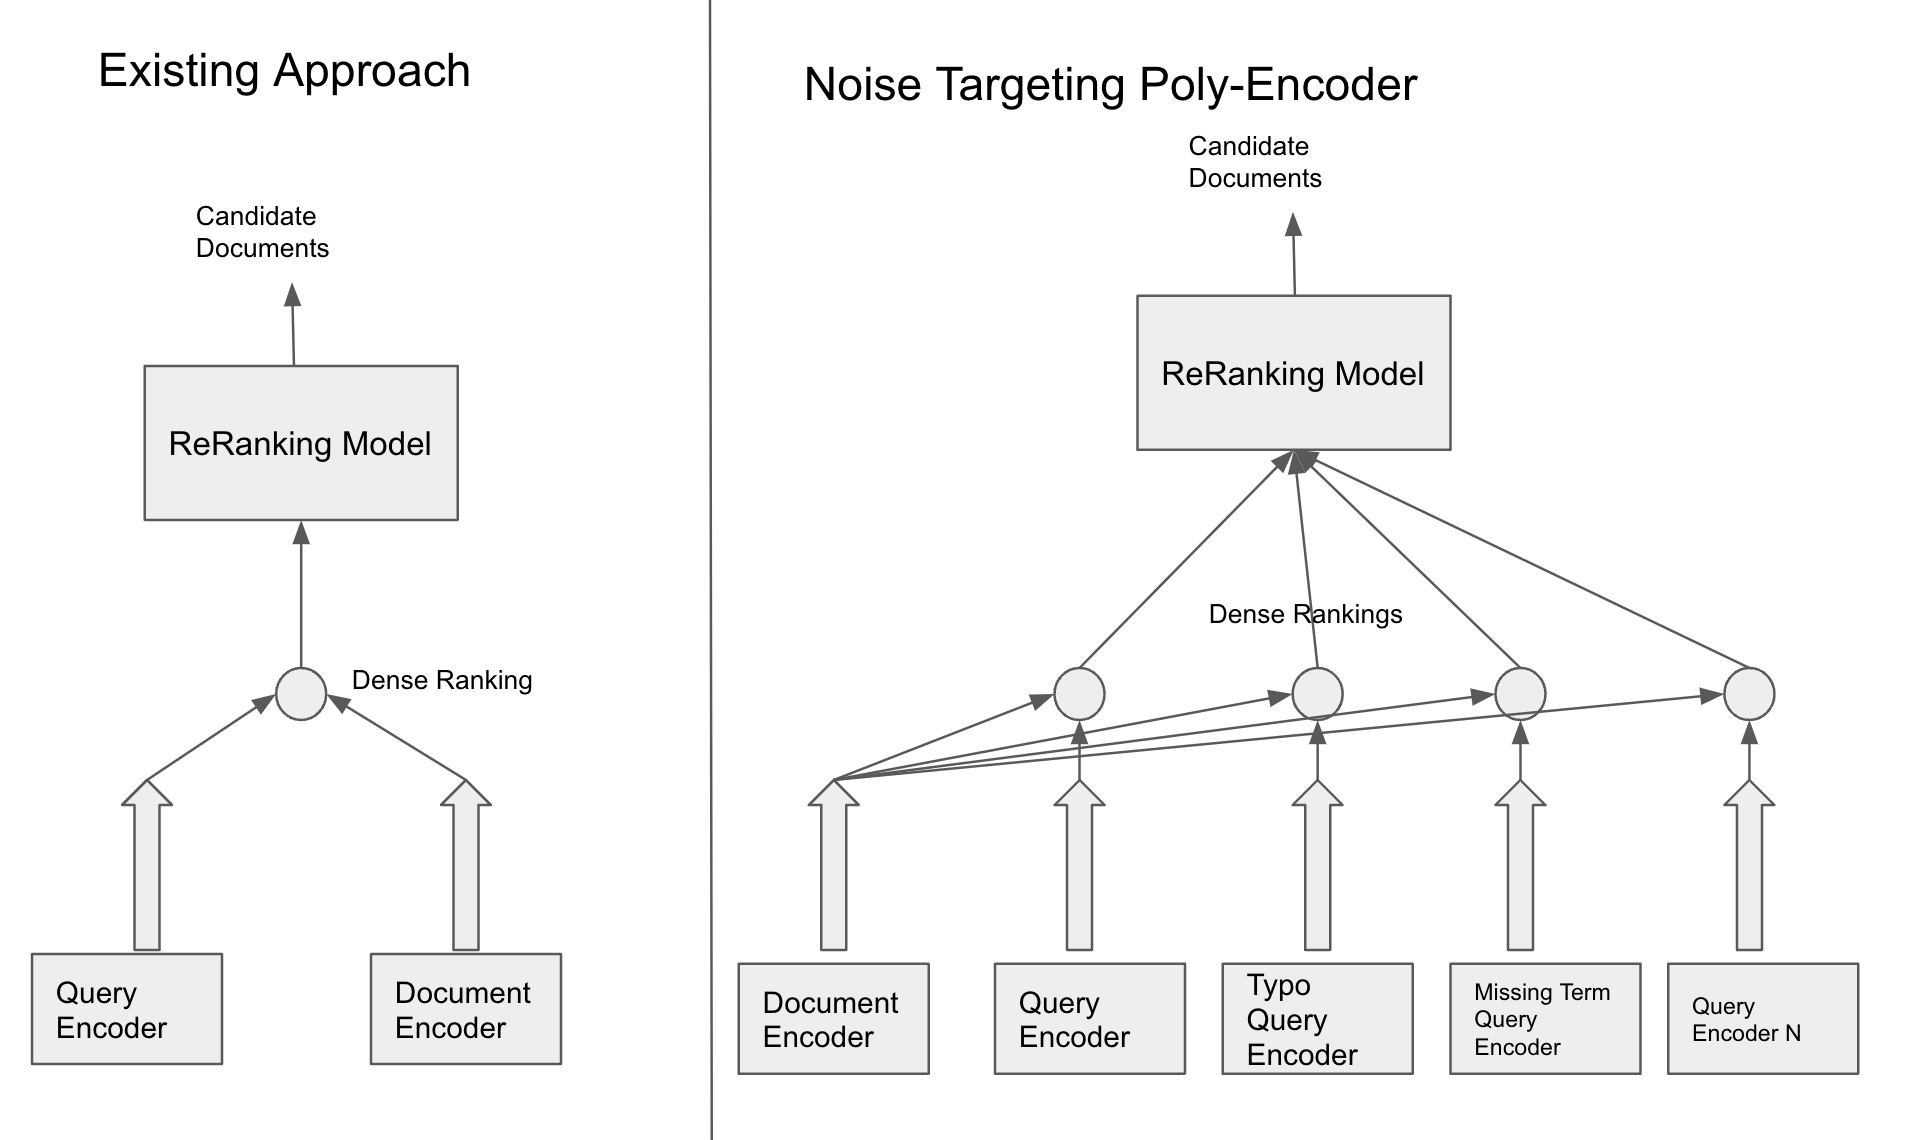
\includegraphics{figure2.png}}
    \caption{Proposed poly-encoder architecture using noise-targeted query encoders optimized with CAPOT}
    \label{fig:fig2}
\end{figure}